\chapter{Goal Oriented Action Planning}
\label{chap:goap}

Das folgende Kapitel wird Goal Oriented Action Planning beschreiben. Es gehört zu den \hyperref[chap:entscheidungssysteme]{Entscheidungssystemen} in der Game-AI und besteht aus dem A* Suchalgorithmus. Es ist für die Planung an Aktionen zu einem bestimmten Ziel gedacht. Planung ist der Prozess der Suche einer Sequenz an Aktionen zur Erreichung eines Zieles. Die Suche kann dabei als Suchproblem dargestellt werden und durch Suchalgorithmen gelöst werden. Für das Verständnis wird daher Kenntnis der Themen Suchalgorithmen und Suchprobleme\ref{} empfohlen.

\section{Historie}
\label{chap:goap historie}

Das \hyperref[chap:entscheidungssysteme]{Entscheidungssystem} \textit{Goal Oriented Action Planning} (\textit{GOAP}) entstand in der Entwicklung des Videospiel \textit{F.E.A.R First Encounter Assault Recon (2005)} durch das Entwicklerstudio \textit{Monolith}. Die Entwickler wollten ein Videospiel entwickeln, das wie ein Actionfilm wirkt, mit intensiven Kämpfen. Für die intensiven Kämpfe benötigt man NPC, welche Deckung nehmen, blind feuern, über Fenster springen, Granaten werfen, untereinander kommunizieren und weitere Aktionen ausführen können.

Zuvor nutzte \textit{Monolith} Finite State Machines (\textit{FSM}) als Entscheidungssystem. Den Entwicklern fiel es jedoch zunehmend aufwendig, eine FSM mit neuen Zuständen und den dazugehörigen Aktionen zu erweitern. In einem vorherigen Videospiel \textit{No One Lives Forever (2000)}, wurde veruscht eine dynamische FSM zu implementieren, die sich an Zielzustände anpassen konnte. Allerdings wurde auch diese Lösung als zu unflexibel wahrgenommen. Aus dem Versuch der dynamischen FSM und STRIPS hat Jeff Orkin das GOAP System entwickelt, welches Echtzeitplanung erfüllen soll. Eine der Herausforderungen, mit denen sich Jeff Orkin während der Entwicklung konfrontiert sah, war die Berücksichtigung der Performance.\autocite{retro_fear}



\section{GOAP Bestandteile}
\label{chap:goap bestandteile}

Das GOAP -System basiert dabei auf dem STRIPS System. Wie auch STRIPS besitzt GOAP Ziele, welche einen gewünschten Zustand beschreiben und Goap-Aktion mit Effekten die Zustände ändern können. GOAP sucht nach einer Sequenz an Goap-Aktion, der Aktions-Sequenz, die das Ziel des NPC erreichen kann. Im Sinne von Jeff Orkins geschieht die eigentliche Ausführung der Aktionen über eine Finite State Machine (\textit{FSM}).


\subsection{Finite State Machine in GOAP}
\label{chap:fsm goap}

Das Videospiel \textit{F.E.A.R} benötigt für die Ausführung der Aktionen eine FSM. Die NPCs führen ihre Aktionen durch eine Kombination aus Animationen und Bewegungen aus. Beispielsweise sorgt eine Cover-Aktion dafür, dass der NPC hinter eine Deckung läuft und dort eine Deckungs-Animation abspielt. Eine Shoot-Aktion hingegen aktiviert eine entsprechende Schuss-Animation. Die FSM besteht dabei aus den drei Zuständen GoTo, Animate und UseSmartObject. 
\begin{figure}[h]
  \centering
  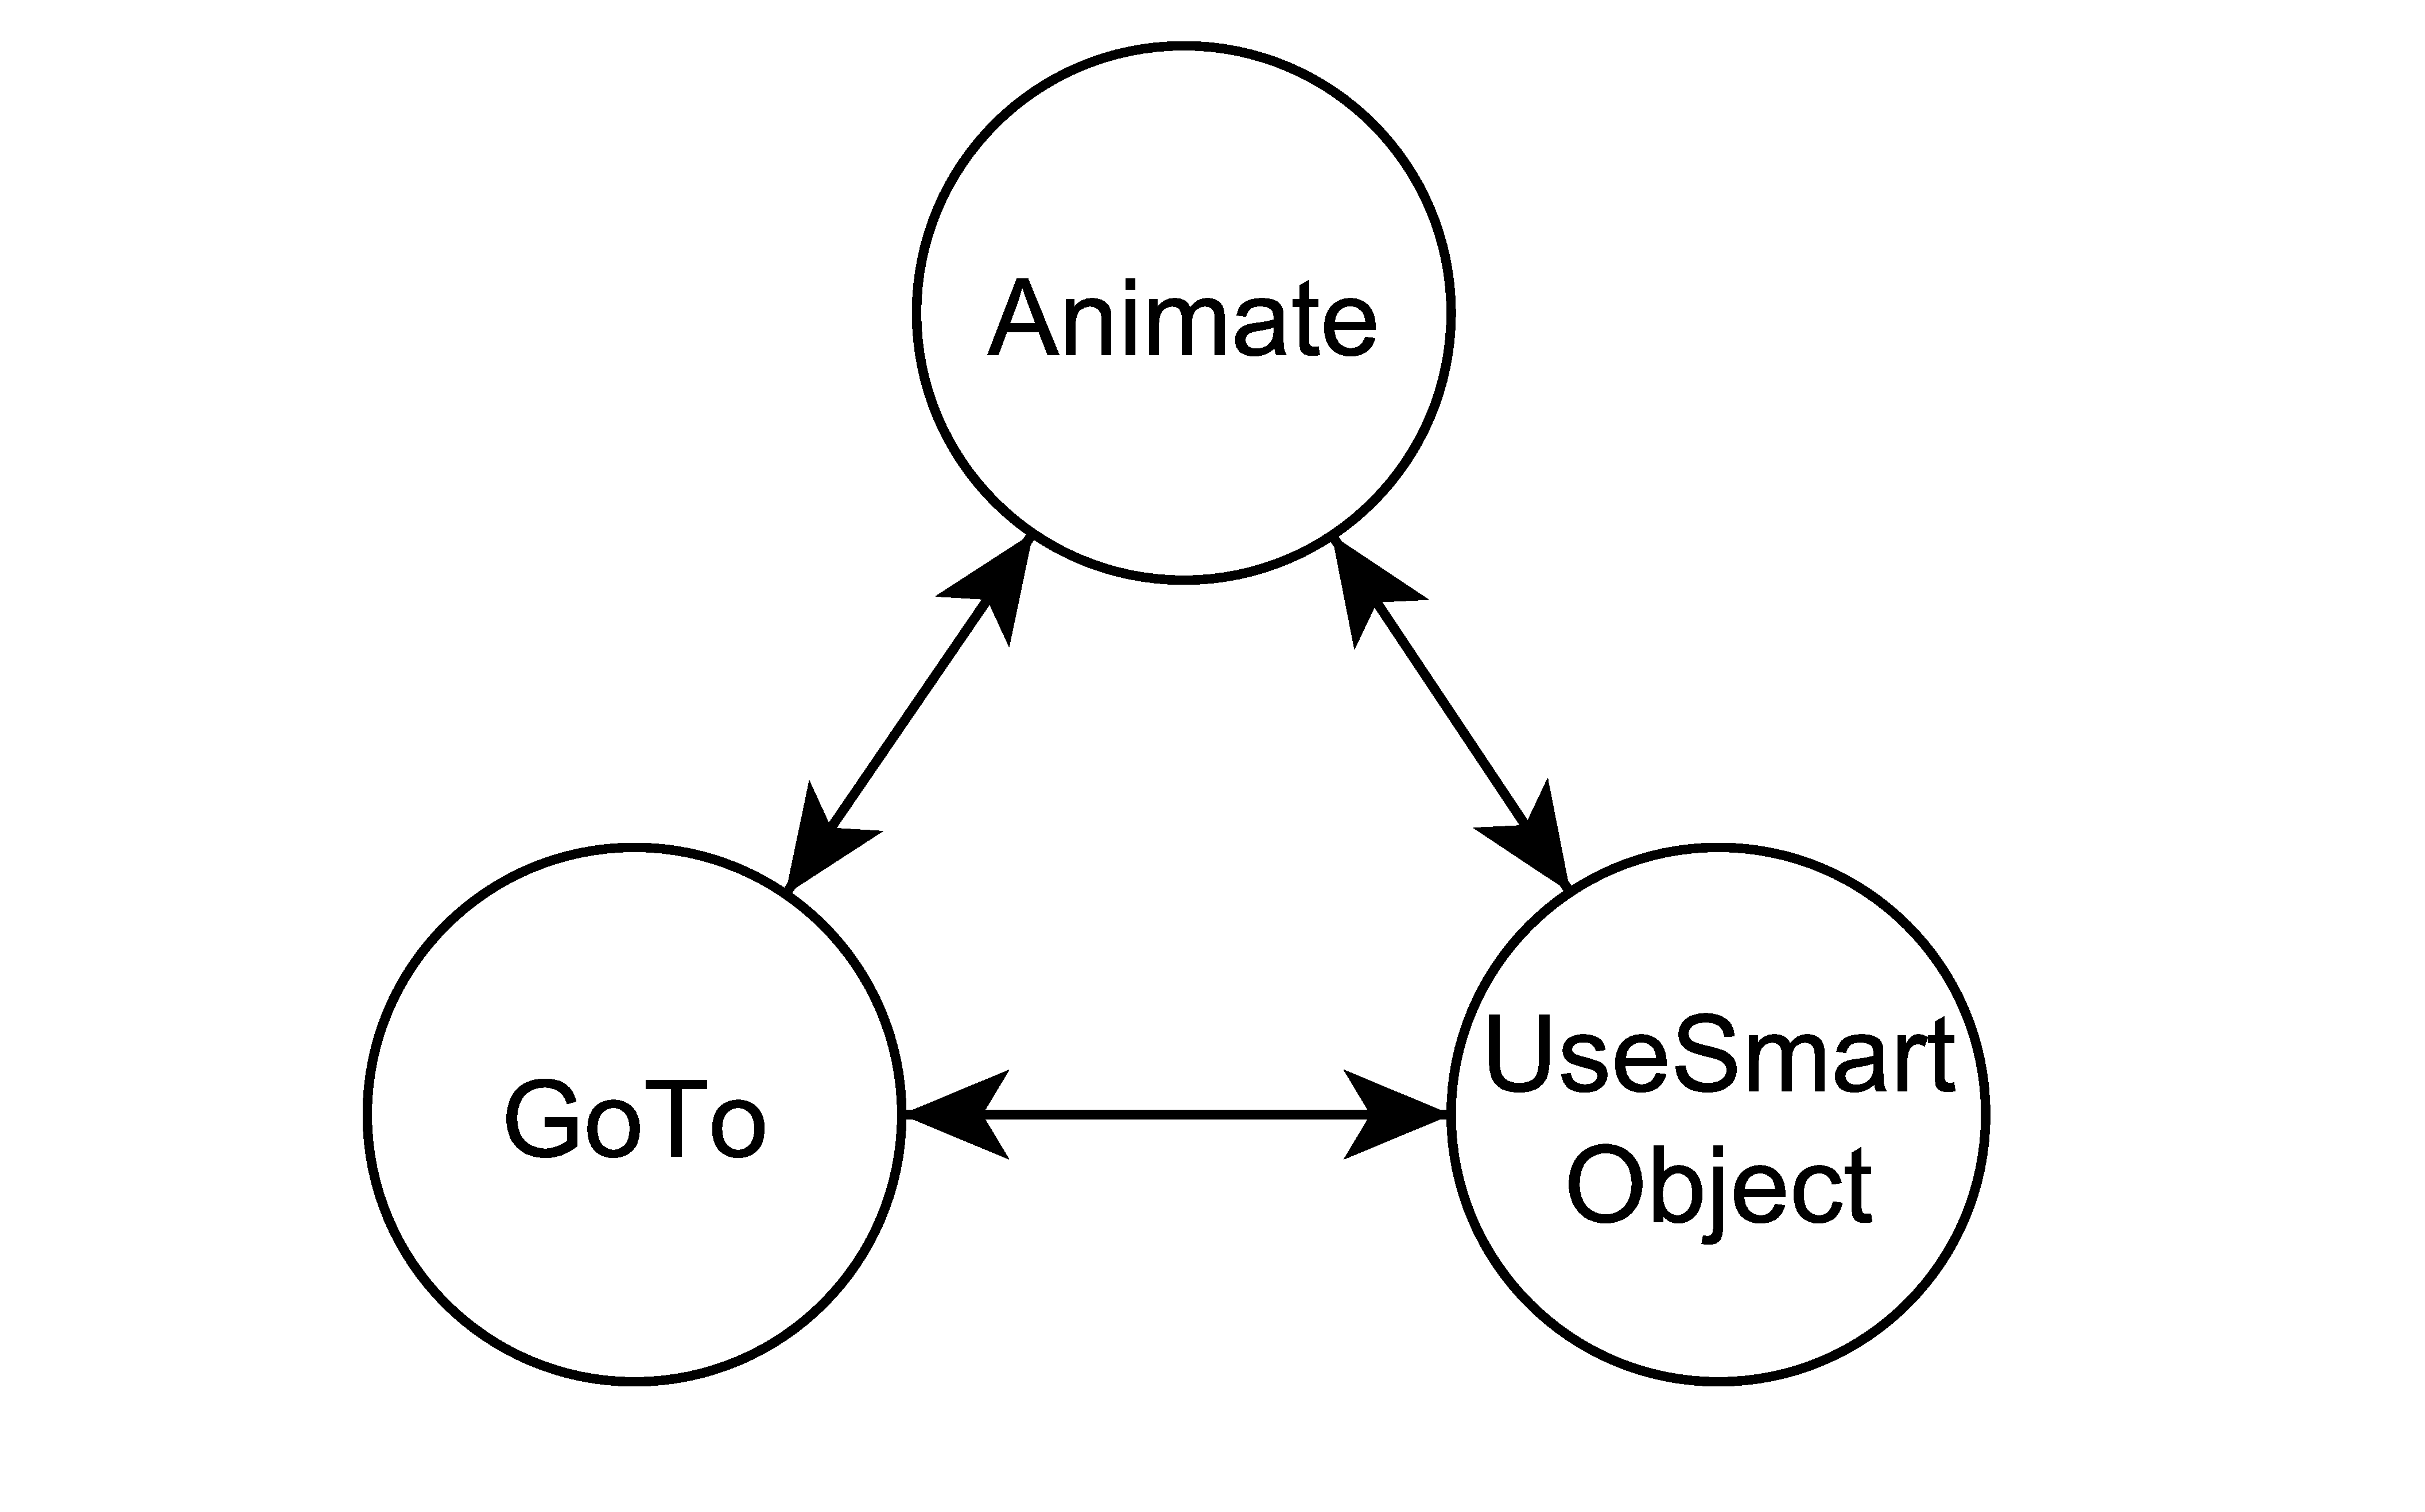
\includegraphics[width=0.7\textwidth]{GOAP/fsm.pdf}
	\captionsetup{justification=justified, format=plain}
  \caption{GOAP Finite State Machine}
  \label{fig:Goap FSM}
\end{figure}

\textit{Monolith} hat durch die Zustände \textit{Animate} und \textit{UseSmartObject} Animationen umgesetzt. Der Unterschied zwischen den beiden Zuständen besteht darin, dass \textit{UseSmartObject} Animationen steuert, die von \textit{SmartObjects} in der Spielwelt vorgegeben werden, während \textit{Animate} Animationen abspielt, die direkt im NPC gespeichert sind. Der Zustand \textit{GoTo} hat ebenfalls Animationen abgespielt, kombiniert diese jedoch mit der tatsächlichen Bewegung des NPCs durch die Spielwelt.

Die Zustandswechsel werden durch die Goap-Aktion bestimmt, welche wiederum durch GOAP gegeben werden.


\subsection{GOAP Ziele}
\label{chap:goap ziele}

Ein Ziel \textit{GOAL}$(g)$ in GOAP setzt die erwünschte Zielzustände für den Planer. So setzt das Ziel \textit{EliminatePlayer} den Zielzustand $\{\lnot \textit{PlayerAlive}\}$.

\begin{align}
	\textit{GOAL}(\textit{EliminatePlayer}) = \{\lnot \textit{PlayerAlive}\}
\end{align}


Die Auswahl des Zieles geschieht nach ihrer Priorität und ob dieses gültig ist. Das Ziel mit der höchsten Priorität und Gültigkeit wird bevorzugt. Die Gültigkeit und Priorität basiert dabei auf dem Zustand $s$ des NPC und seiner Umwelt. So ist das Ziel \textit{EliminatePlayer} mit dem Zustand $s$ nicht gültig und besitzt eine hohe Priorität.

\begin{align}
	s = \{\lnot \textit{PlayerVisible}\} \\
	\textit{PRIORITY}(s,\textit{EliminatePlayer}) = 100 \\
	\textit{VALID}(s,\textit{EliminatePlayer}) = \textit{false}
\end{align}


\subsection{GOAP Aktionen}
\label{chap:goap actions}

Die Goap-Aktion können Weltzustände oder auch direkte Zustände eines NPC ändern. So kann beispielsweise die Goap-Aktion \textit{Reload} den Zustand $s = \{\lnot \textit{GunLoaded}\}$ mit seinem Effekt ändern.

\begin{align}
	\textit{TRANSITIONS}(s,\textit{Reload}) &= \{\textit{GunLoaded}\}
\end{align}


Dadurch haben Goap-Aktion die Möglichkeit Zielzustände zu erreichen. Man nehme an, dass der NPC das Ziel \textit{Patrol} verfolgt, mit dem gewünschten Zustand \textit{AtPatrol}, und dass die Aktion \textit{GoPatrol} den Effekt \textit{TRANSITIONS}$(s, \textit{GoPatrol}) = {\textit{AtPatrol}}$ hat. In diesem Fall kann die Goap-Aktion durch ihren Effekt den gewünschten Zielzustand erreichen.

Eine Goap-Aktion hat auch Vorbedingungen als Zustände, diese Zustände können wiederum von anderen Goap-Aktionen erfüllt werden. So kann beispielsweise die Goap-Aktion \textit{Reload} die Vorbedingung der Goap-Aktion \textit{Shoot} erreichen.

\begin{align}
	\textit{PRECONDITION}(\textit{Shoot}) = \{\textit{GunLoaded}\}
\end{align}

Eine Goap-Aktion setzt auch wie im Suchproblem\ref{} eine \textit{ACTIONCOST} Funktion um, die später zur Auswahl einer Goap-Aktion herangezogen wird. Wird die Goap-Aktion ausgewählt wird diese später von der FSM ausgeführt.


\subsubsection{Fallbeispiel}
\label{chap:goap action beispiel}

Nehmen wir an, dass der NPC den Ausgangszustand $s_a$ und das Ziel \textit{EliminatePlayer} besitzt.

\begin{align}
	s_a = \{\textit{PlayerVisible}, \lnot \textit{GunLoaded}\, \lnot \textit{AtCover}\} \\
	\textit{GOAL}(\textit{EliminatePlayer}) = \{\lnot \textit{PlayerAlive}\}
\end{align}


Der NPC muss nun versuchen das Ziel mit den möglichen Goap-Aktion den Zielzustand $\{\lnot \textit{PlayerAlive}\}$ erreichen. Die möglichen Goap-Aktion werden dafür aus einer $\textit{ACTIONS}(s)$ Funktion gelesen.

\begin{align}
	\textit{ACTIONS}(s) = \{\textit{Reload}, \textit{MoveToCover}\} \\
	\textit{TRANSITIONS}(s,\textit{Reload}) = \{\textit{GunLoaded}\} \\
	\textit{TRANSITIONS}(s,\textit{MoveToCover}) = \{\textit{AtCover}\}
\end{align}


Aus der \textit{TRANSITIONS} Funktion können wir entnehmen, dass keine der Goap-Aktion den Zustand $\lnot \textit{PlayerAlive}$ direkt erreichen kann. Es muss ein Zustand entdeckt werden aus dem mit einer entsprechenden Goap-Aktion das Ziel erreicht werden kann. Eine Lösung wäre \textit{Brute Force}, das durchgehen aller möglichen Goap-Aktion bis letztlich das Ziel gefunden wird. Dies sorgt jedoch für einen hohen Rechenaufwand bei komplexen NPC mit vielen Goap-Aktion und Zuständen. Außerdem können beim Brute Force suboptimale Aktions-Sequenzen gefunden werden, da dieser die Kosten der Goap-Aktion nicht beachtet. In GOAP sucht der A*-Suchalgorithmus über den GOAP Planner die optimale Aktions-Sequenz.


\subsection{GOAP Planner}
\label{chap:goap planner}

Der GOAP Planner ist dabei die eigentliche Lösung des Suchproblems. Der Planner bestimmt das Ziel mit der höchsten Priorität und Gültigkeit. Die dazugehörige Aktions-Sequenz wird über den A*-Suchalgorithmus im GOAP Planner gesucht. Der A*-Suchalgorithmus\ref{} wird im Kapitel Suchalgorithmen ausführlich beschrieben.

\subsubsection{Knoten und Kanten}
\label{chap:goap knoten und kanten}

Der A*-Suchalgorithmus ist in der Videospiel-Entwicklung für die Suche des Navigation-Pfades bekannt. Er kann aber auch für andere Suchprobleme genutzt werden, wie für die Suche einer Aktion-Sequenz. Wie auch für die Navigation erzeugt der A*-Suchalgorithmus einen Suchbaum, mit dem Unterschied, dass die Knoten Zustände des NPC sind, die durch die Kanten also Goap-Aktionen erzeugt werden.

Knoten speichern die nicht erfüllten Zustände des NPC für das erreichen des Zieles ab, während Kanten die Goap-Aktionen darstellen die von einem Knoten zu einem neuen Knoten führen.

\begin{table}[h]
  \caption{A* Vergleich: Navigation und Aktions-Plannung}
  \label{A*: Vergleich}
  \renewcommand{\arraystretch}{1.2}
  \centering
  \small
    \begin{tabularx}{0.95\textwidth}{X X X}
      \toprule
      \textbf{A*} & \textbf{Navigation} & \textbf{Aktion-Plannung}\\
      \midrule
      Knoten & NavMesh Polygon & Zustand &
			Kanten & NavMesh Polygon Kanten & Goap-Aktionen &
      \bottomrule
    \end{tabularx}
\end{table}


\subsubsection{Bewertungsfunktion}
\label{chap:goap bewertungsfunktion}

Die Bewertungsfunktion des A*-Suchalgorithmus setzt sich aus $f(n) = g(n) + h(n)$ zusammen. In GOAP ist $g(n)$ die Funktion $\textit{ACTIONCOST}(s,a,s^*)$, welche die Kosten der Kante darstellt, also die Kosten für die Ausführung der Goap-Aktion $a$, die vom Zustand $s$ zum Zielzustand $s^$ führt. Die Heuristik $h(n)$ wird durch die Summe der noch nicht erfüllten Zustände des jeweiligen Knotens dargestellt. Je geringer der Wert von $h(n)$, desto näher ist der Knoten dem Ziel. 


\subsubsection{Suche der Aktions-Sequenz}
\label{chap:goap suche}

Es ist zwar möglich aus dem Ausgangszustand zu suchen, könnte aber einem \textit{Brute Force}\ref{} ähneln und dadurch ineffizient sein. Die Kante wird nicht wie bei der Navigation vom Ausgangszustand ausgewählt, sondern aus dem Zielzustand $s_z$ aus. Von dort aus wird die Suche nach Kanten fortgesetzt, die die Vorbedingungen der zuvor gewählten Kante erfüllen. Die Suche wird fortgesetzt bis alle Vorbedingungen der Kanten erfüllt wurden. Der Planer speichert dabei die Auswahl der Goap-Aktionen in einer Aktions-Sequenz ab.


\section{Suchbeispiel}
\label{chap:goap suchbeispiel}

Wir setzten das Beispiel mit dem Wissen über den GOAP Planner fort. Dabei definiert $s_a$ den Ausgangszustand des NPC.

\begin{align}
	s_a = \{\textit{PlayerAlive}, \textit{PlayerVisible}, \lnot \textit{AtPatrol}, \lnot \textit{GunLoaded}\, \\
	\lnot \textit{AtCover}, \lnot \textit{AtPlayer},  \lnot \textit{AtLastPlayerPostion}\}
\end{align}


\subsubsection{Auswahl des Zieles}
\label{chap:goap ziel auswahl}

\begin{table}[h]
  \caption{Ziel Tabelle}
  \label{Kap4:Ziel}
  \renewcommand{\arraystretch}{1.2}
  \centering
  \small
    \begin{tabularx}{0.95\textwidth}{X X X R}
      \toprule
      \textbf{Goal} & \textbf{Ziel-Zustand} & \textbf{Gültigkeit} & \textbf{Priorität}\\
      \midrule
      EliminatePlayer & \lnot \text{PlayerAlive} & PlayerVisible & 3 \\
			SearchEnemy & AtLastPlayerPostion & \lnot \text{AtLastPlayerPostion} & 2 \\
			Patrol & \lnot \text{AtPatrol} & AtLastPlayerPostion & 1 &
      \bottomrule
    \end{tabularx}
\end{table}

Der GOAP Planer wählt das Ziel mit der höchsten Priorität und Gültigkeit. Nehmen wir an, dass das Ziel \textit{Patrol} aufgrund der \textit{VALID(s,Patrol)} Funktion nicht gültig ist, so würde das Ziel ausfallen. Es verbleiben die Ziele: \textit{EliminatePlayer} und \textit{SearchEnemy}. Da \textit{EliminatePlayer} mit $\textit{PRIORTIY}(s,\textit{EliminatePlayer}) = 3$ die höhere Priorität hat, wird diese als Ziel ausgewählt.

\subsubsection{Suche nach der Aktion-Sequenz}
\label{chap:goap suche nach aktionen}

\begin{table}[h]
  \caption{Aktionen ihre Effekte und Vorausgesetzte Zustände}
  \label{Kap4:Aktionen}
  \renewcommand{\arraystretch}{1.2}
  \centering
  \small
    \begin{tabularx}{0.95\textwidth}{l l l l}
      \toprule
      \textbf{Aktion} & \textbf{Effekt} & \textbf{Vorausgesetzte Zustände} & \textbf{Kosten}\\
      \midrule
      Shoot & \lnot \text{PlayerAlive} & GunLoaded, PlayerVisible & 1\\
			Melee & \lnot \text{PlayerAlive} & AtPlayer, PlayerVisible & 3\\
      Reload & GunLoaded & \lnot \text{GunLoaded} & 1\\
      GoTo & AtCover, AtPlayer, AtLastPlayerPostion & - & 0-10 &
      \bottomrule
    \end{tabularx}
\end{table}


Der Algorithmus erstellt nun einen Suchbaum. Der Wurzelknoten im Suchbaum speichert, dabei den erwünschten Zielzustand des Zieles. Im Falle des Beispiels ist der Zielzustand $s_z = \textit{GOAL}(\textit{EliminatePlayer}) = \{\lnot \textit{PlayerAlive}\}$.

\begin{figure}[h]
  \centering
  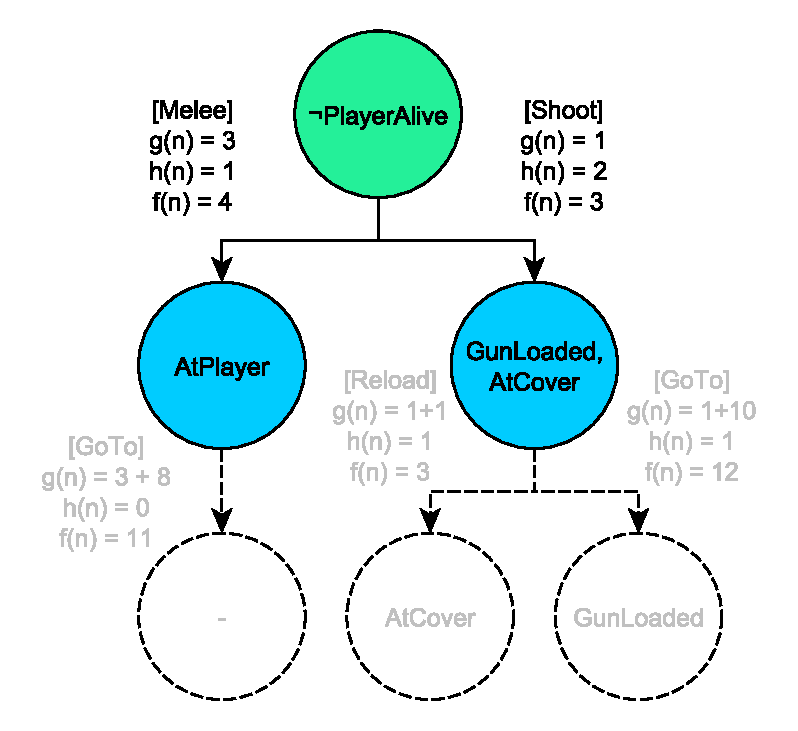
\includegraphics[width=0.5\textwidth]{GOAP/goap baum 1}
	\captionsetup{justification=justified, format=plain}
  \caption{GOAP A* Suche: Grüne Knoten sind Knoten, welche erweitert wurden. Blaue Knoten sind Knoten aus der offenen Liste.}
  \label{fig:goap1}
\end{figure}

Nun sucht der Planner alle möglichen Aktionen die den Zielzustand erreichen ($\textit{ACTIONS}(s_z) = {\textit{Shoot}, \textit{Melee}}$). Es werden nicht erfüllte und vorausgesetzte Zustände der gefundenen Aktionen, sowie die Kosten $g(n)$ und $f(n)$ in den Knoten hinterlegt. Beide werden in die offene Liste hinzugefügt.

Zur weiteren Suche entscheidet sich der A* Algorithmus für den Knoten mit den geringsten Kosten aus der offenen Liste, welcher durch die Bewertungsfunktion $f(n) = g(n) + h(n)$ berechnet wurde. Die Kosten $g(n)$ werden durch die $\textit{ACTIONCOST}$-Funktion gelesen. Die Heuristik $h(n)$ stellt sich durch die Summe an noch nicht erfüllten Zuständen. Im Beispiel expandiert A* den Knoten \textit{GunLoaded, AtCover} der durch die Aktion \textit{Shoot} generiert wurde. Der Zustand \textit{AtPlayer} bleibt weiterhin in der offenen Liste.

\begin{figure}[h]
  \centering
  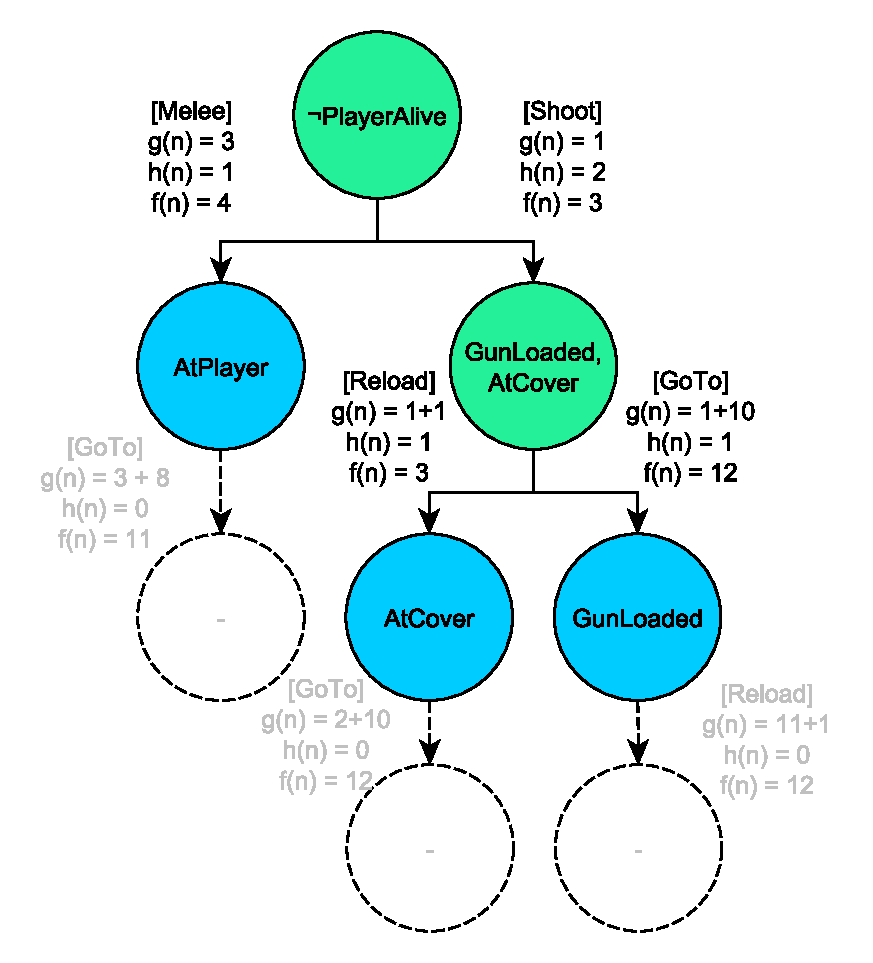
\includegraphics[width=0.6\textwidth]{GOAP/goap baum 2}
	\captionsetup{justification=justified, format=plain}
  \caption{GOAP A* Suche}
  \label{fig:goap2}
\end{figure}

Für den expandierten Knoten \textit{GunLoaded, AtCover} werden nun Aktionen gesucht, die die Zustände des Knoten erfüllen. In dem Beispiel sind es \textit{Reload} und \textit{GoTo}. Auch die Knoten die durch die Aktionen entstehen, werden in die offene Liste hinzugefügt. Erneut wählt A* den Knoten mit den geringsten Kosten $f(n)$ zur Expansion.
\clearpage

\begin{figure}[h]
  \centering
  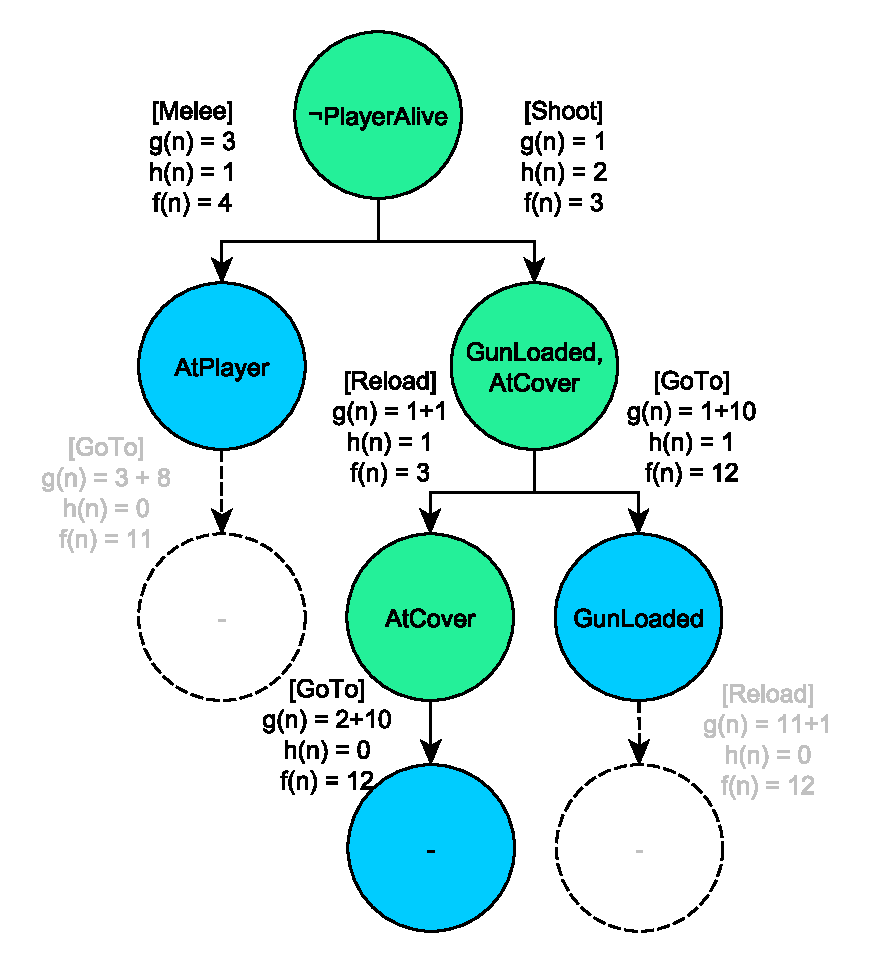
\includegraphics[width=0.6\textwidth]{GOAP/goap baum 3}
	\captionsetup{justification=justified, format=plain}
  \caption{GOAP A* Suche}
  \label{fig:goap3}
\end{figure}

Der Knoten der durch die Aktion \textit{Reload} entstand, hat dabei die geringsten $f(n)$ Kosten. Der nachfolgende Knoten, der durch die Aktion \textit{GoTo} erzeugt wird, hat zwar einen leeren Zustand und wäre somit abgeschlossen, befindet sich jedoch gemeinsam mit dem \textit{AtPlayer}-Knoten, der geringere Kosten hat, noch in der offenen Liste.

\begin{figure}[h]
  \centering
  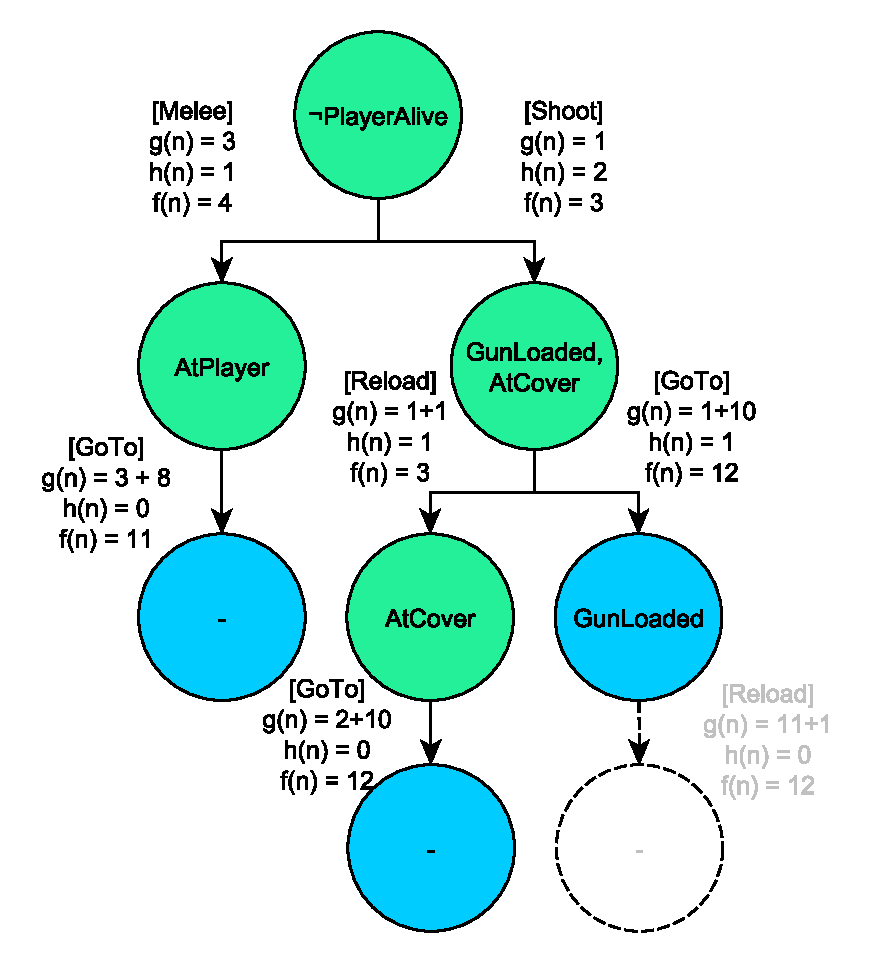
\includegraphics[width=0.6\textwidth]{GOAP/goap baum 4}
	\captionsetup{justification=justified, format=plain}
  \caption{GOAP A* Suche}
  \label{fig:goap4}
\end{figure}

Aus der offenen Liste wird der nächste Knoten mit dem Zustand \textit{AtPlayer} gewählt, da dieser die niedrigsten Kosten von allen anderen offenen Knoten hat. Dieser wird durch die Aktion \textit{GoToPlayer} erfüllt und führt zu einem Knoten mit leerem Zustand.

\begin{figure}[h]
  \centering
  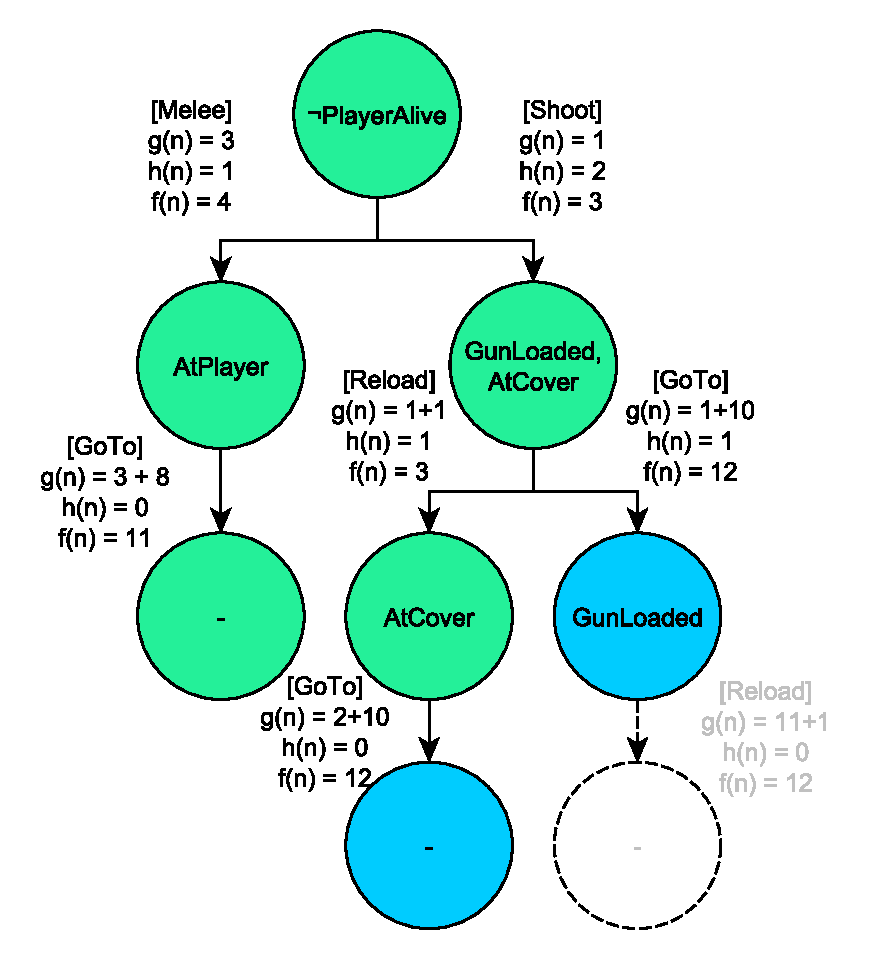
\includegraphics[width=0.6\textwidth]{GOAP/goap baum final}
	\captionsetup{justification=justified, format=plain}
  \caption{GOAP A* Suche}
  \label{fig:goap5}
\end{figure}

Letztlich wird der günstigste Knoten aus der offenen Liste genommen. Da dieser erfüllt ist, beziehungsweise keine weiteren Zustände besitzt, gibt der Planner nun die Goap-Aktionen, also die Kanten, die zu ihm geführt habe in einer Aktions-Sequenz zurück. Im Beispiel wäre es die Aktions-Sequenz: [\textit{Melee, GoTo}]. Diese Aktions-Sequenz muss nun gespiegelt werden, da der A*-Suchalgorithmus vom Zielzustand angefangen hat. Somit wäre die richtige Aktions-Sequenz: [\textit{GoToPlayer, Melee}].